\chapter{相關文獻探討}

\section{同步建模}

\subsection{隱形參數}
在看了同步建模的演示後,許多人會認為方向盤的功能太神奇了,透過方向盤的變化,就能將3D模型玩弄於股掌中,不需要輸入參數,就可以隨心所欲地進行模型的設計,但其實這是錯的,畢竟Solid Edge也是由人類藉由科學的力量開發出來的,而不用參數所設計出來的軟體是不存在的,只是用這種方向盤的方式讓參數的變化更自由,而導致有人沒發現而已。\\

以圖\ref{2.79}為例,將方向盤拖動綠色平面往右邊移動時,可以透過選取模型的邊界來讓系統自動確定移動的距離,當從原平面拖移時,系統會檢測且紀錄所選的平面到原始平面位置的距離,這些是由Solid Edge在後台完成,所以說同步建模還是有帶參數的設計過程,只是表面上看不太出來而已。\\
\begin{figure}[hbt!]
\begin{center}
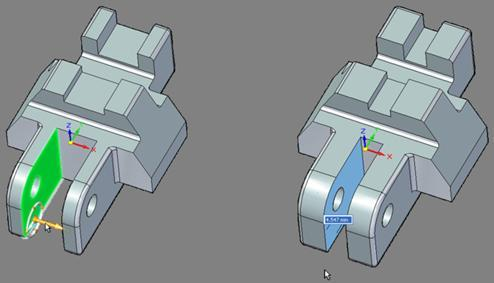
\includegraphics[width=10cm]{同步建模演示1}
\caption{\Large 同步建模方向盤}\label{2.79}
\end{center}
\end{figure}
\\

同步建模環境的參數操控比一般建模更加方便且迅速,可以控制參數變化的方向,這比一般建模裡必須依賴約束關係來操控參數變化方向更加的直覺,且能在不需進到草圖的情況下,直接移動模型的邊和面來達到參數的變化,能節省下設計變更的時間。\\
以圖\ref{2.80}為例,如需將30mm的間距修改的話,可以選擇通過移動肋板或是移動外殼的外型來達成,而且只需要簡單的用滑鼠點擊兩方的箭頭即可。\\
\begin{figure}[hbt!]
\begin{center}
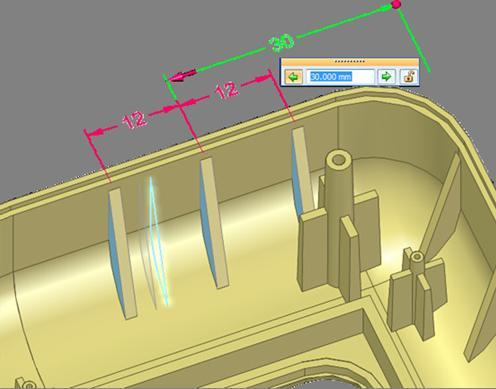
\includegraphics[width=10cm]{同步建模演示2}
\caption{\Large 同步建模參數變化}\label{2.80}
\end{center}
\end{figure}
\\
\subsection{自由度}

同步建模可以隨心所欲,彷彿没有規律可循,方向盤利用滑鼠拖移到哪邊,零件就會立即發生相對應的變化,好像就可以隨意設計一樣。但並非這樣的,再拖移方向盤時,Solid Edge系統會時刻檢測操控的動作,同時系統所隱含的設計規則一直在保障模型的變化,只符合和設定的設定規則的模型圖素材會發生變化,在Solid Edge中將此變化稱之為及時規則,這種技術在傳統建模裡是沒有的,這就是同步建模的魅力所在!\\

\subsection{特徵樹}

在同步建模的有些操作後,不會發生特徵樹的變化,比如拖動方向盤、旋轉方向盤,但不代表同步建模可以不要特徵樹,同步建模是採納傳統順序建模基於特徵的優勢,並没有抛棄特徵。\\

在傳統順序建模裡,特徵具有嚴格的時間歷史順序,這樣對設計者就提出要求,在設計之前就必須要預先規劃好設計過程,否則就會產生意想不到的结果,而且改了特徵樹前面的草圖及特徵後,後續所有的特徵都需要重新計算,如果不是經驗老到的工程師,能讓規畫好的設計過程來減少更改特徵的次數的話,就會讓導致系統產生大量的等待時間。但特徵樹的好處則在於他會清晰記錄你的所有操作步驟,可以很方便地找到特徵,然後進行修改。\\

同步建模則採納了特徵的這些優勢保留下来,捨棄了它的缺點,就是將歷史的概念去除,讓所有的特徵都在同一層。當在修改其中某一特徵時,所有與之相關的特徵一起發生了變化,而不相關的特徵則保持不變,這樣就極大的提高了效率,且減少了大量的運算時間。 \\

在同步特徵樹下,可以通過按名稱排序,還是類型排序,模型都不會發生任何變化。在拖動方向盤的时候,只不過是對其中部分特徵進行修改,所以也不會再產生新的特徵樹。\\

因此同步建模的特徵模式更加符合設計的特點。\\

\subsection{特徵參數}

用多了同步建模方向盤的操作,任何修改都可以用方向盤來實現,而不去修改特徵參數。但其實在同步建模環境中,我們既可以用方向盤的拖曵、旋轉、定向來執行對模型的修改,也可以直接編輯特徵草圖裡的參數,來達成一樣的目標,硬生生地比傳統的建模方式多了一種設計方式。\\

這些特徵在同步建模環境裡統稱為過程特徵,如螺旋拉伸/除料、陣列、孔、螺旋、鈑金中的沖型、補強肋、...。\\

修改圖\ref{2.81}中的陣列,只需要選擇這個特徵,系統就會自動彈出這個特徵的所有參數,如陣列類型、個數、填充方式等,比起傳統建模的修改方式還方便許多。\\
\begin{figure}[hbt!]
\begin{center}
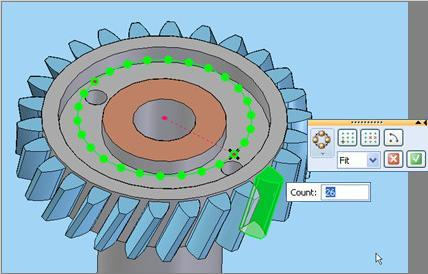
\includegraphics[width=10cm]{同步建模演示3}
\caption{\Large 同步建模過程特徵}\label{2.81}
\end{center}
\end{figure}
\\
\subsection{幾何約束}

習慣了傳統建模的方式,習慣將幾何約束添加在2D草圖,現在在同步建模裡幾何約束也能添加在3D環境下,但同步建模僅僅是有3D的幾何約束,也保留了傳統建模裡的2D幾何約束,各自有各自的工作,名負其責。\\

圖\ref{2.82}是在3D環境下的幾何約束。通過同心、對稱、偏移、共面、相切等等約束關係,直接加載在3D模型的面上,所以說3D約束是控制模型的面。\\
\begin{figure}[hbt!]
\begin{center}
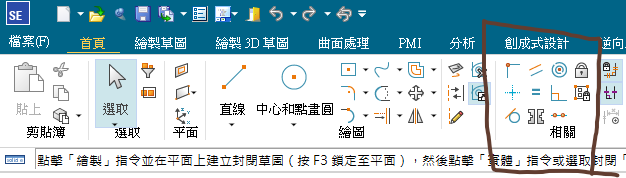
\includegraphics[width=12cm]{同步建模演示4}
\caption{\Large 同步建模3D幾何約束}\label{2.82}
\end{center}
\end{figure}
\\
\qquad 圖\ref{2.83}是在2D繪圖環境下的幾何約束。雖然功能的名稱是一樣的,但只能加載在2D圖形上,也就是點和線,所以說2D約束是控制2D的點和線,不能控制到3D幾何的面。\\
\begin{figure}[hbt!]
\begin{center}
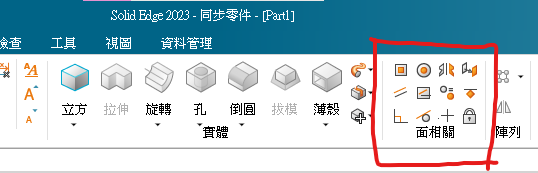
\includegraphics[width=12cm]{同步建模演示5}
\caption{\Large 同步建模2D幾何約束}\label{2.83}
\end{center}
\end{figure}
\\

\qquad 兩者相比,因為肉眼能直接看到模型的變化,不須像傳統建模一樣,要先在大腦有個底,所以3D幾何約束比起2D的幾何約束更加直覺、直接地控制模型變化,這是同步建模在CAD建模技術上的一大突破。\\

\qquad 而同步建模環境,既可以添加2D幾何约束,也能添加3D幾何約束。\\

\newpage


\section{工程參照}

工程參照是Solid Edge的一種特有功能,直覺來說就是快速建模,只需要選擇需要的模型形狀,再將數值一一打入,即使不用畫草圖也能迅速的將模型產生。\\

\subsection{設計器}

在工作列上的工具裡能很輕易的找到工程參照,點開有高達13項的模型提供選擇。\\
\begin{figure}[hbt!]
\begin{center}
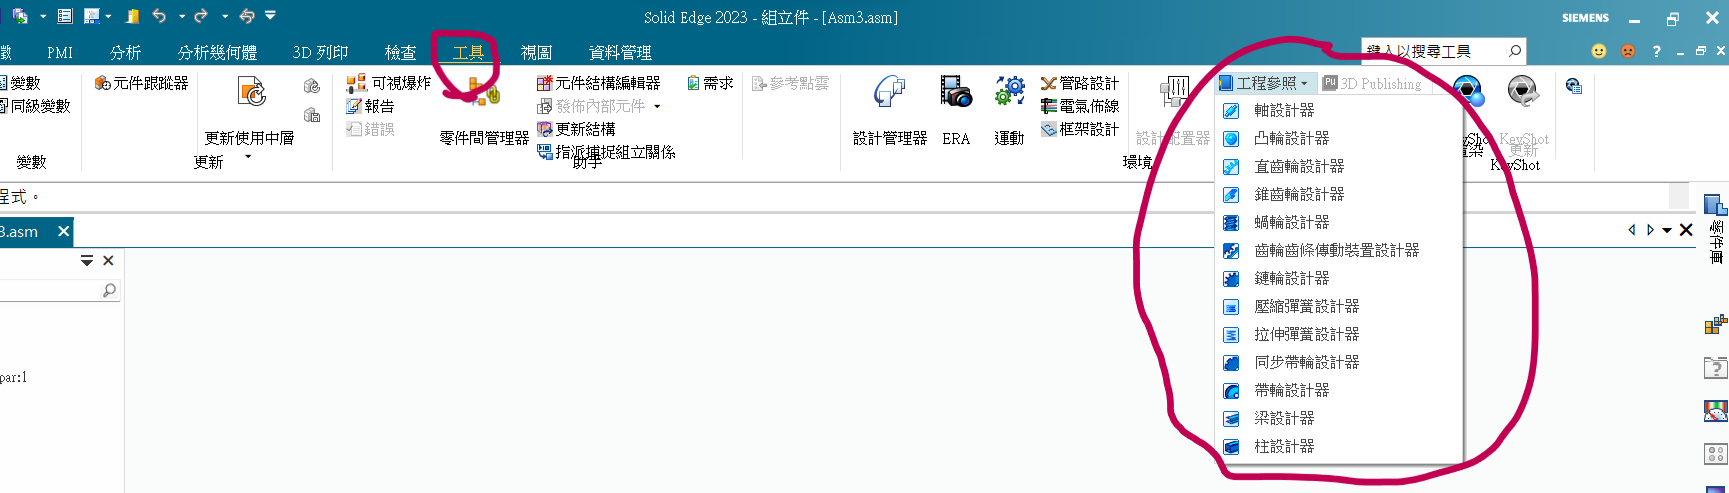
\includegraphics[width=16cm]{螢幕擷取畫面 2023-05-11 200432}
\caption{\Large 開啟位置}\label{開啟位置}
\end{center}
\end{figure}
\\
開啟(圖.\ref{開啟畫面}):\\

每種模型的界面都大同小異,有各個尺寸的代號、參數調整,因為還能算出簡易的分析,所以也有支撐(固定)、負載與設定材質的功能,模型預覽的功能因只能做出較簡單的畫面變更,所以只有軸設計器與梁設計器有而已。\\
\begin{figure}[hbt!]
\begin{center}
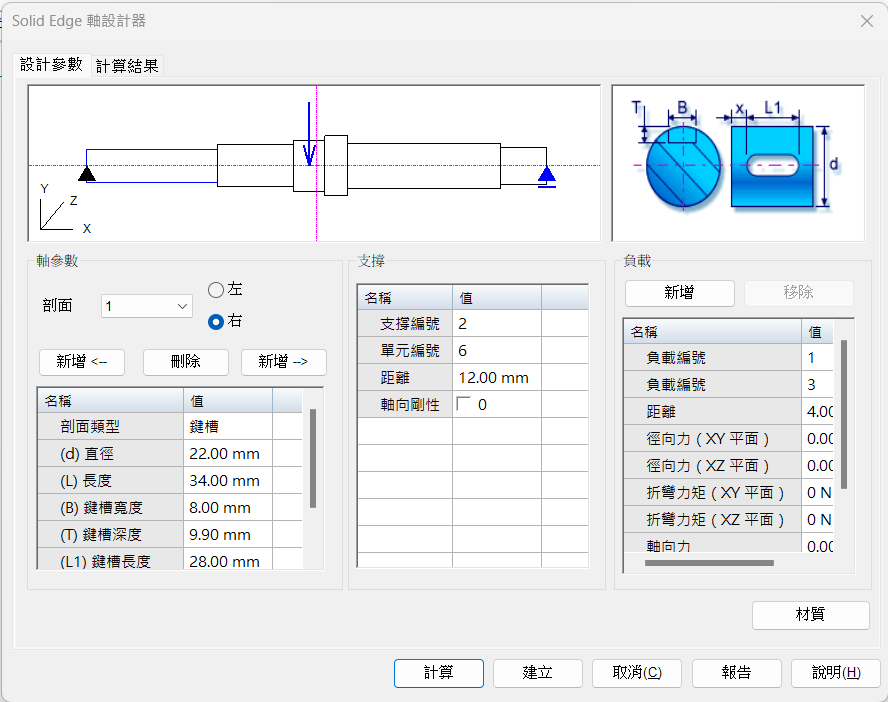
\includegraphics[width=12cm]{軸設計器1}
\caption{\Large 開啟畫面}\label{開啟畫面}
\end{center}
\end{figure}
\\
材質(圖.\ref{材質畫面}、圖.\ref{內建材質}):\\

模型材質的更改,有提供常用的材料可以選擇,如果沒有需要的材料的話也能透過彈性模量(楊氏係數)、剛性模量及比值量來達成設定。\\
\begin{figure}[hbt!]
\begin{center}
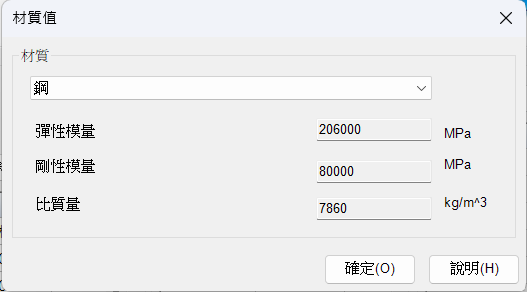
\includegraphics[width=8cm]{軸設計器6}
\caption{\Large 材質畫面}\label{材質畫面}
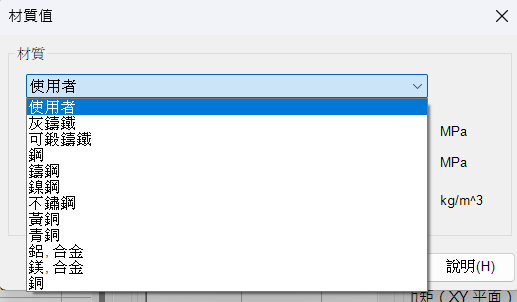
\includegraphics[width=8cm]{螢幕擷取畫面 2023-05-11 205001}
\caption{\Large 內建材質}\label{內建材質}
\end{center}
\end{figure}
\\

分析結果(圖.\ref{分析結果畫面}):\\

設定參數完成後,按下計算就能直接得到力的分析結果,各種力作用及平面都能自由調整來得到需要的數值。\\
\begin{figure}[hbt!]
\begin{center}
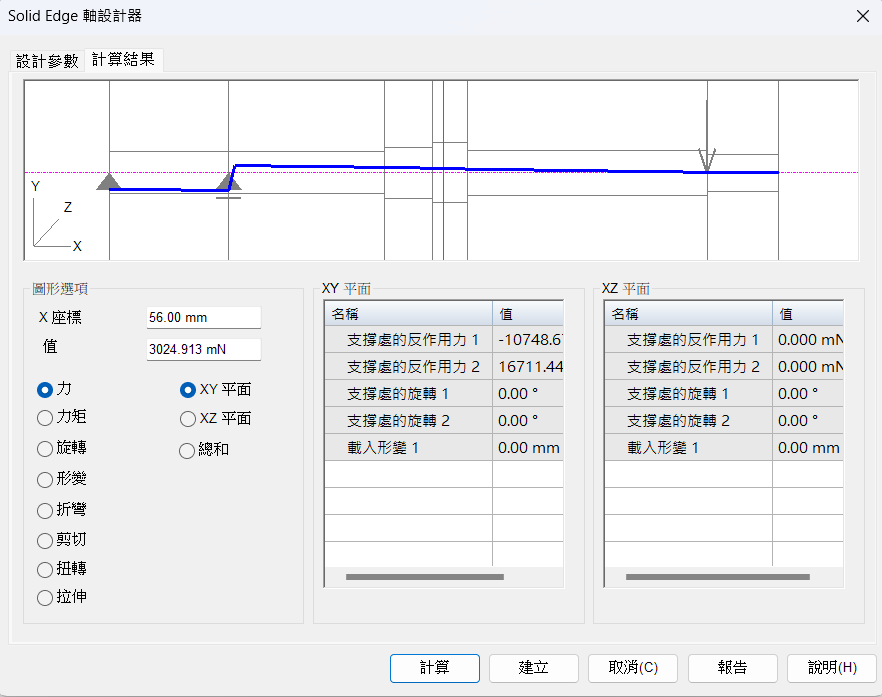
\includegraphics[width=12cm]{軸設計器7}
\caption{\Large 分析結果畫面}\label{分析結果畫面}
\end{center}
\end{figure}
\\

以下介紹工程參照的各種設計器:
\begin{itemize}
		%=----------Sigmoid      Function----------=%
	\item 軸設計器(圖.\ref{軸設計器}):\\
	
		\qquad 在做參數設計只需要打上想要的尺寸即可得到想要的模型,上面預覽所呈現的藍線部分就是對應到下面軸參數的數值,也能隨時改變剖面的類型,自由度非常的高,但須注意的是預覽部分並不會將各個剖面的類型顯現出來,所以預覽的畫面並非是建立出來的完整模型\\

		\qquad 支撐功能裡的支撐編號是預覽畫面中的藍色三角形,左邊的三角形是程式預設的固定邊,而右邊的三角形會根據單元編號的改變所移動,支撐編號只有1(預設固定邊)與2(單元編號)提供選擇\\

		\qquad 負載功能也有一些相較簡單的力能輸入,力的位置也會顯示在預覽畫面上,材質部分也有預設一些比較常用到的材料,如果沒有的話,也只要將需要的材料性質輸入進去即可\\
		\begin{figure}[hbt!]
		\begin{center}
		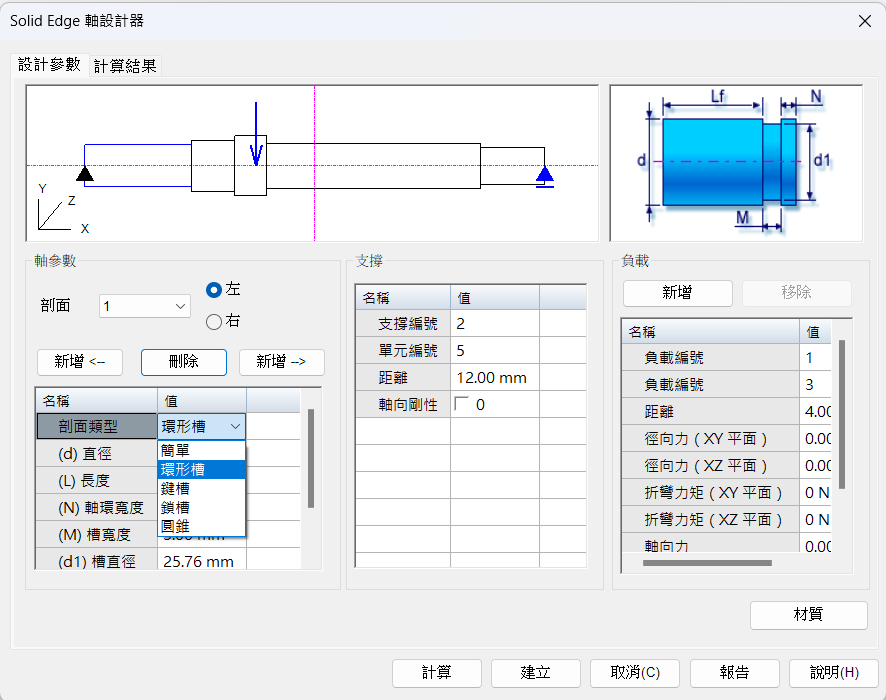
\includegraphics[width=12cm]{軸設計器2}
		\caption{\Large 軸設計器}\label{軸設計器}
		\end{center}
		\end{figure}
		\\
		剖面選擇的數值是模型從左到右開始算的第幾個剖面(圖.\ref{剖面選擇})
		\begin{figure}[hbt!]
		\begin{center}
		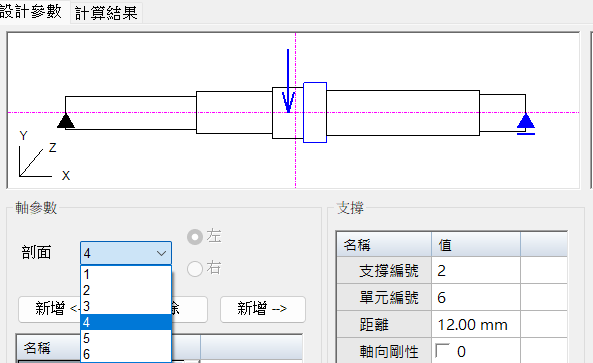
\includegraphics[width=12cm]{00}
		\caption{\Large 剖面選擇}\label{剖面選擇}
		\end{center}
		\end{figure}
		\\
		新增的功能就是在所選擇的剖面左/右邊新增新的剖面(圖.\ref{2.8})\\
		\begin{figure}[hbt!]
		\begin{center}
		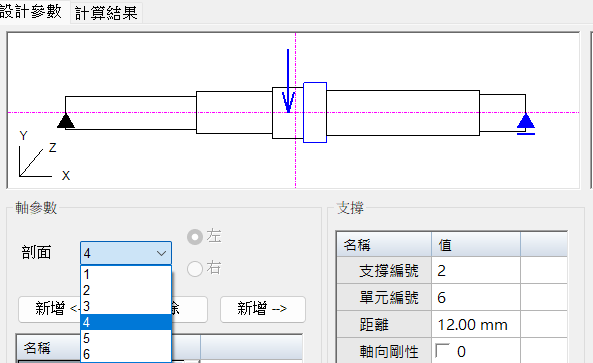
\includegraphics[width=12cm]{00}
		\caption{\Large 新增}\label{2.8}
		\end{center}
		\end{figure}
		\\
		計算結果(圖.\ref{2.9})
		\begin{figure}[hbt!]
		\begin{center}
		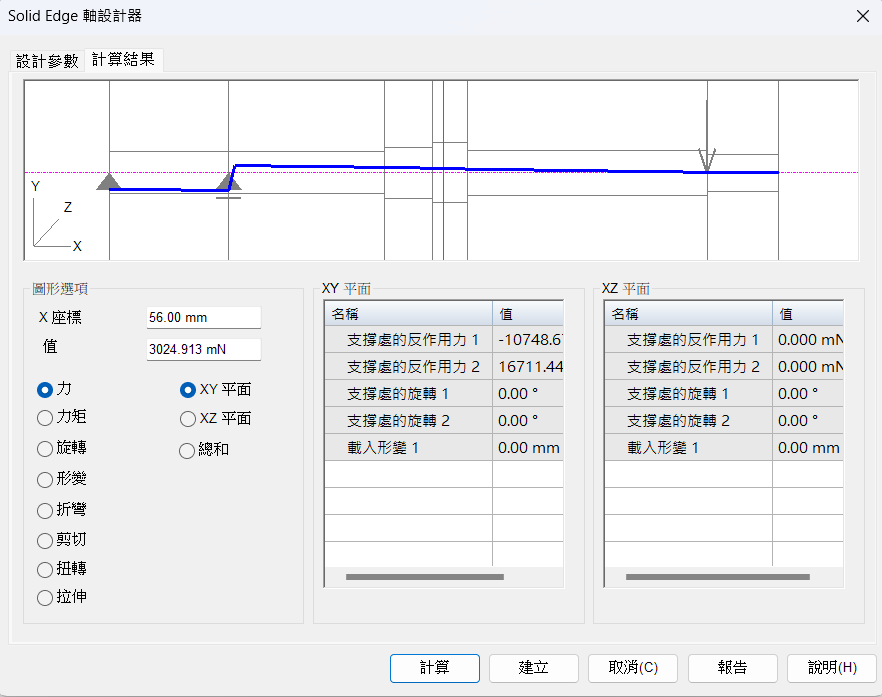
\includegraphics[width=12cm]{軸設計器7}
		\caption{\Large 記算結果}\label{2.9}
		\end{center}
		\end{figure}
		\\
		模型建立(圖.\ref{2.10})
		\begin{figure}[hbt!]
		\begin{center}
		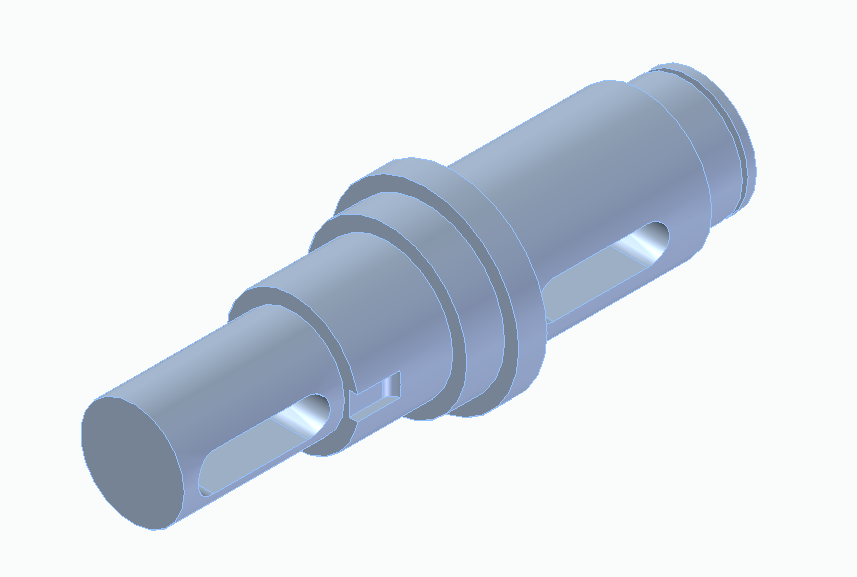
\includegraphics[width=10cm]{軸模型}
		\caption{\Large 軸模型}\label{2.10}
		\end{center}
		\end{figure}
		\\
		
\newpage

	
	\item 凸輪設計器(圖.\ref{2.11}) :\\
	
		\qquad 與軸設計器相同,一樣有著參數以及負載的數值可以輸入,上面畫面一樣是各數值所代表的部位,而在凸輪參數最下列還有一項周速的數值是不可調整的,是直接經由上列數值所計算出來的
		\begin{figure}[hbt!]
		\begin{center}
		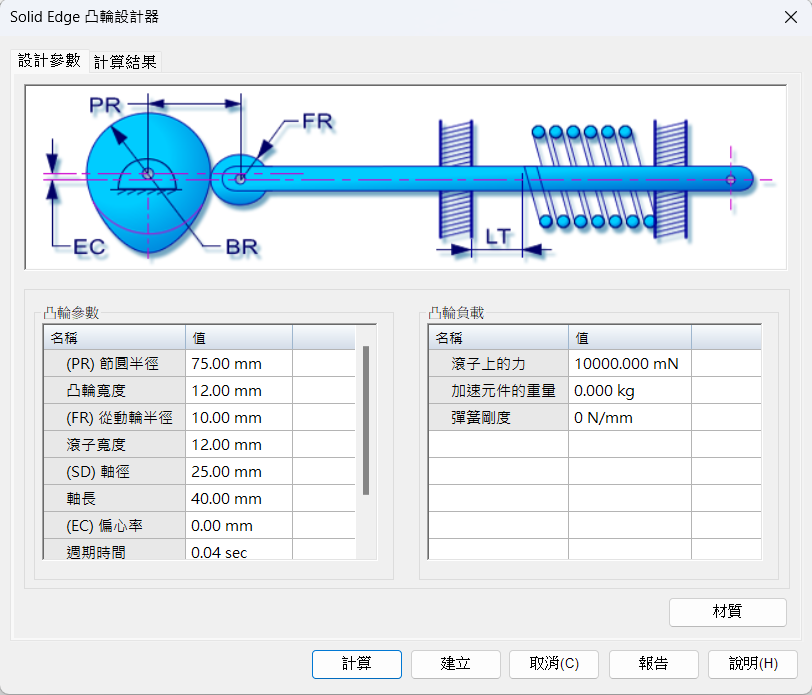
\includegraphics[width=12cm]{凸輪1}
		\caption{\Large 凸輪設計器}\label{2.11}
		\end{center}
		\end{figure}
		\\
		材質(圖.\ref{2.12})
		\begin{figure}[hbt!]
		\begin{center}
		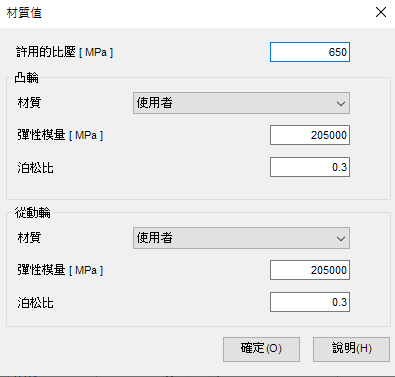
\includegraphics[width=8cm]{禿倫}
		\caption{\Large 凸輪材質}\label{2.12}
		\end{center}
		\end{figure}
		\\
		計算結果(圖.\ref{2.13})\\
		
		\qquad 點擊計算後會來到計算結果的頁面,左上畫面是左下角圖形選項的結果,有位移、速度、加速度和躍度提供選擇;而右上的圖形是設計參數計算出來的凸輪輪廓,藍色線是基圓紅色線則是凸輪的形狀;在來是段的選擇,總共有3段的選項,分別是1(0°~120°)、2(120°~240°)、3(240°~360°)
		\begin{figure}[hbt!]
		\begin{center}
		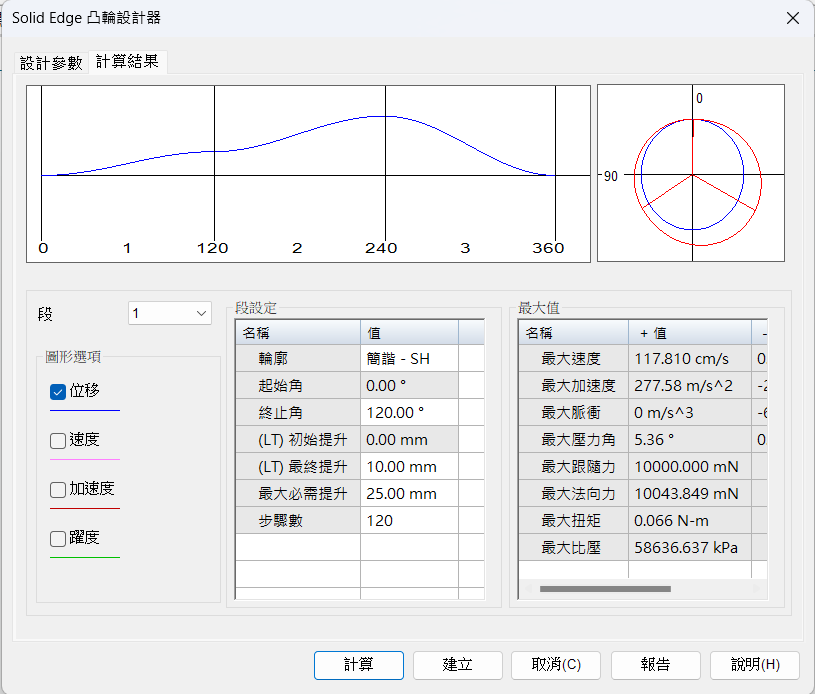
\includegraphics[width=12cm]{凸輪2}
		\caption{\Large 凸輪計算結果}\label{2.13}
		\end{center}
		\end{figure}
		\\
		
		\qquad 各段的設定也都是可以各別做調整的,右邊也會有一些常用的最大數值及時計算出來提供參考(圖.\ref{2.14}、圖.\ref{2.15}、圖.\ref{2.16})
		\begin{figure}[hbt!]
		\begin{center}
		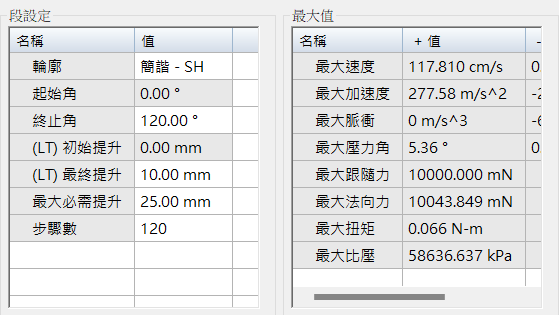
\includegraphics[width=10cm]{凸輪4}
		\caption{\Large 凸輪0°-120°}\label{2.14}
		\end{center}
		\end{figure}
		\\
		\begin{figure}[hbt!]
		\begin{center}
		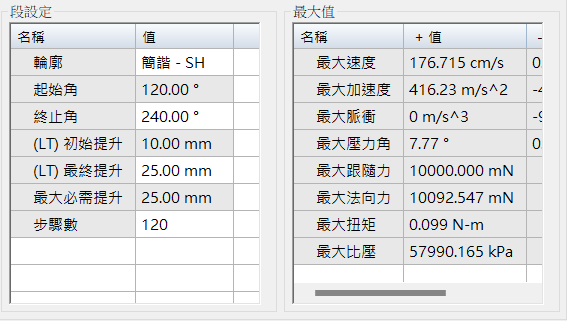
\includegraphics[width=10cm]{凸輪5}
		\caption{\Large 凸輪120°-240°}\label{2.15}
		\end{center}
		\end{figure}
		\\
		\begin{figure}[hbt!]
		\begin{center}
		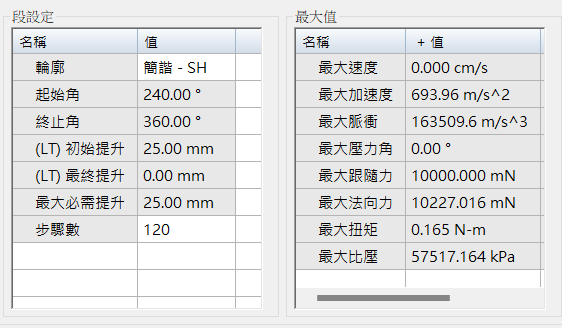
\includegraphics[width=10cm]{凸輪6}
		\caption{\Large 凸輪240°-360°}\label{2.16}
		\end{center}
		\end{figure}
		\\
		模型建立(圖.\ref{2.17})
		\begin{figure}[hbt!]
		\begin{center}
		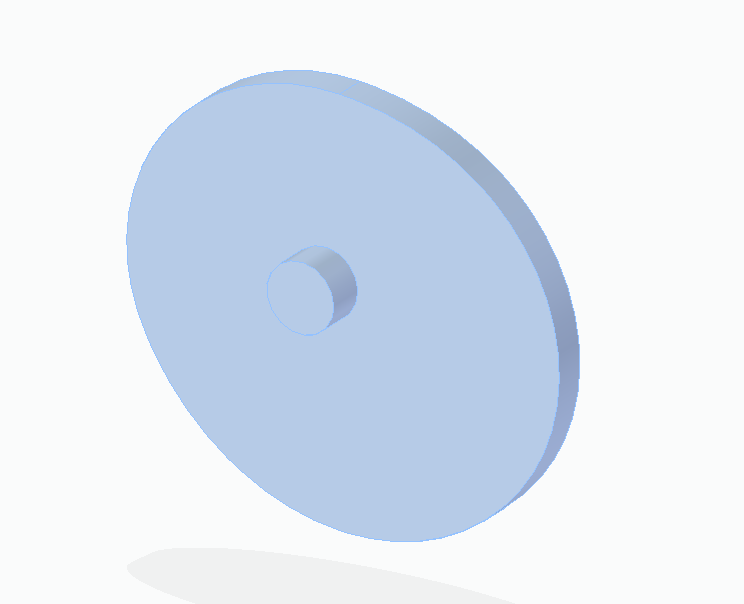
\includegraphics[width=1cm]{凸輪模型}
		\caption{\Large 凸輪模型}\label{2.17}
		\end{center}
		\end{figure}
		\\
		
\newpage
	
	\item 直齒輪設計器(圖.\ref{2.18}) :\\
	
		\qquad 開啟畫面一樣是分成3大部分,代號部位介紹、齒輪參數和計算參數
		\begin{figure}[hbt!]
		\begin{center}
		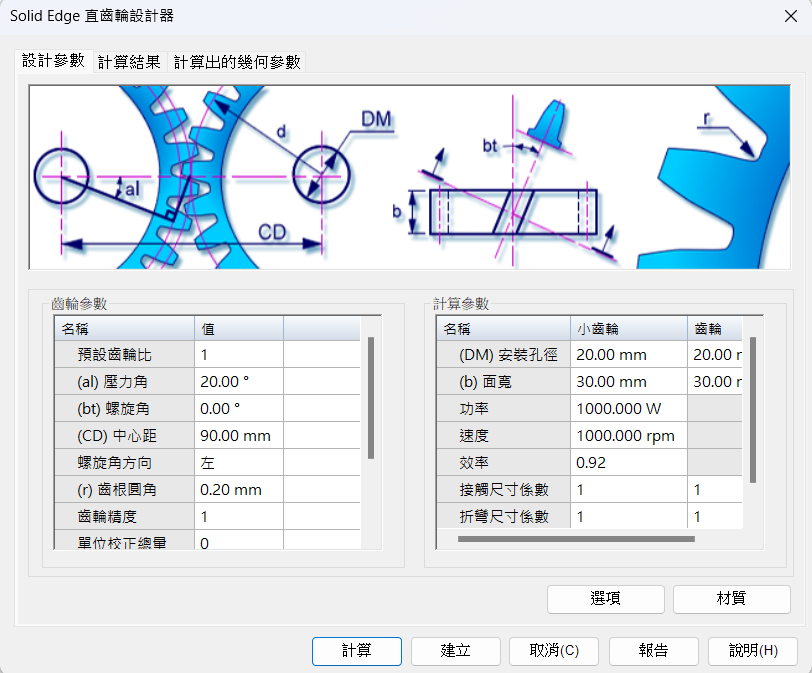
\includegraphics[width=12cm]{直齒輪1}
		\caption{\Large 直齒輪設計器}\label{2.18}
		\end{center}
		\end{figure}
		\\
		選項(圖.\ref{2.19})\\
		參數設計的輸入條件\\
		\begin{figure}[hbt!]
		\begin{center}
		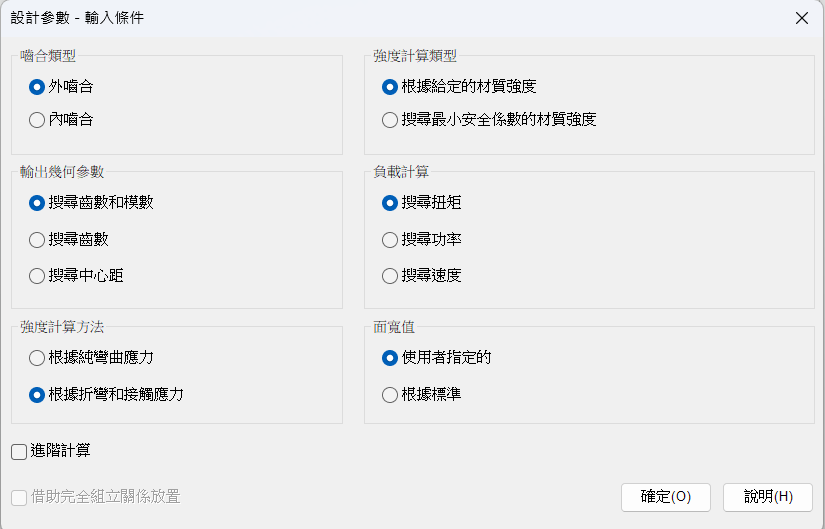
\includegraphics[width=10cm]{螢幕擷取畫面 2023-05-18 200646}
		\caption{\Large 細部選項}\label{2.19}
		\end{center}
		\end{figure}
		\\
		計算結果(圖.\ref{2.20})\\
		\qquad 計算結果這邊因設計器的預設是設計一組齒輪的,所以結果會呈現兩顆齒輪聶合的基本資訊,也會有兩顆齒輪在運動時所產生的各向力作用,以及強度驗證的通過與否\\
		\begin{figure}[hbt!]
		\begin{center}
		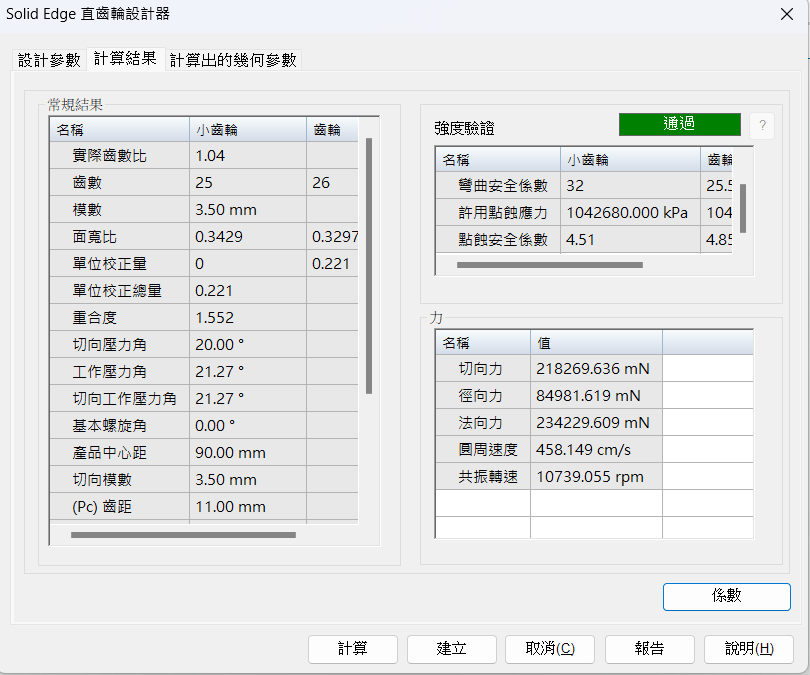
\includegraphics[width=12cm]{直齒輪5}
		\caption{\Large 直齒輪計算結果}\label{2.20}
		\end{center}
		\end{figure}
		\\
		係數(圖.\ref{2.21})\\
		計算後結果的各項係數\\
		\begin{figure}[hbt!]
		\begin{center}
		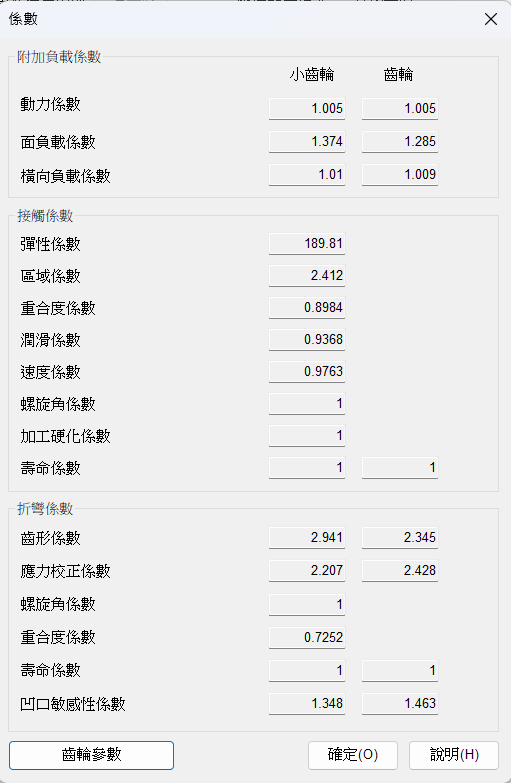
\includegraphics[width=8cm]{直齒輪6}
		\caption{\Large 直齒輪計算結果係數}\label{2.21}
		\end{center}
		\end{figure}
		\\
		齒輪參數(圖.\ref{2.22})\\
		\begin{figure}[hbt!]
		\begin{center}
		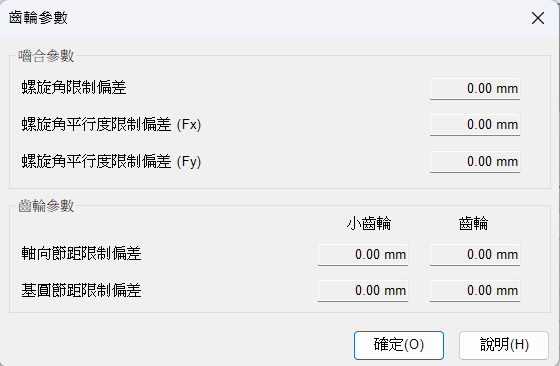
\includegraphics[width=8cm]{直齒輪7}
		\caption{\Large 係數齒輪參數}\label{2.22}
		\end{center}
		\end{figure}
		\\
		計算出的幾何參數(圖.\ref{2.23})\\
		\qquad 各項設定計算出來的幾何參數,也是齒輪最終各部位的基本尺寸\\
		\begin{figure}[hbt!]
		\begin{center}
		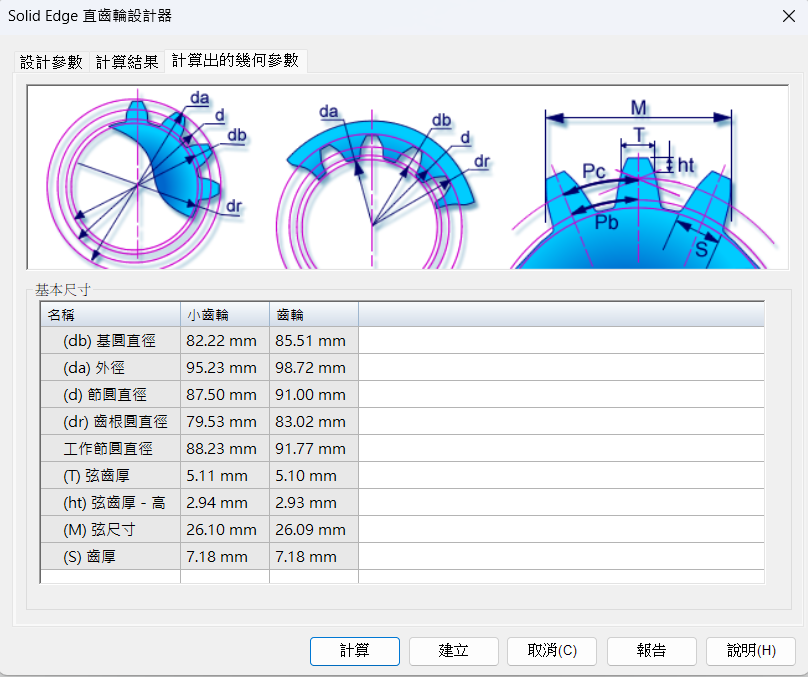
\includegraphics[width=12cm]{直齒輪8}
		\caption{\Large 直齒輪幾何參數}\label{2.23}
		\end{center}
		\end{figure}
		\\
		建立模型(圖.\ref{2.24})\\
		\begin{figure}[hbt!]
		\begin{center}
		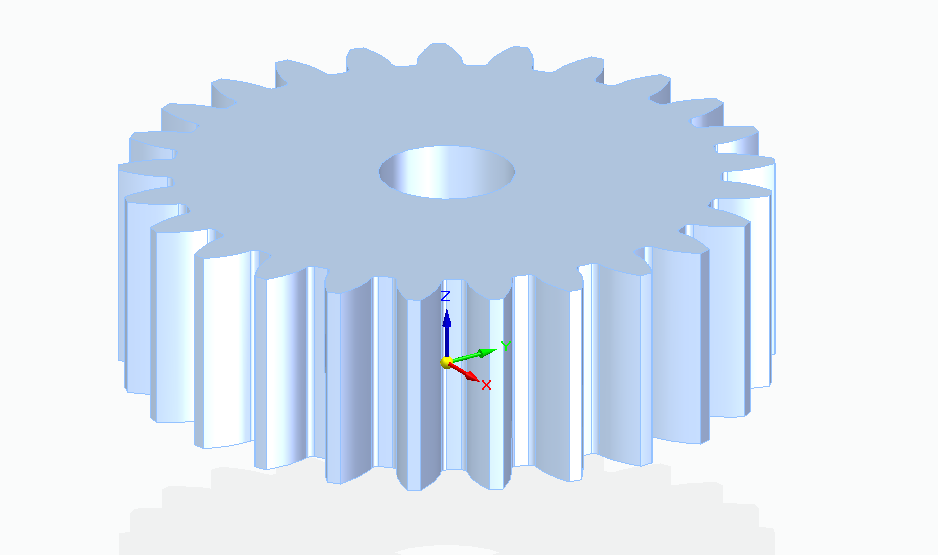
\includegraphics[width=10cm]{正齒輪模型}
		\caption{\Large 直齒輪模型}\label{2.24}
		\end{center}
		\end{figure}
		\\
		
\newpage
		
	\item 錐齒輪設計器(圖.\ref{2.25}) :\\
		\begin{figure}[hbt!]
		\begin{center}
		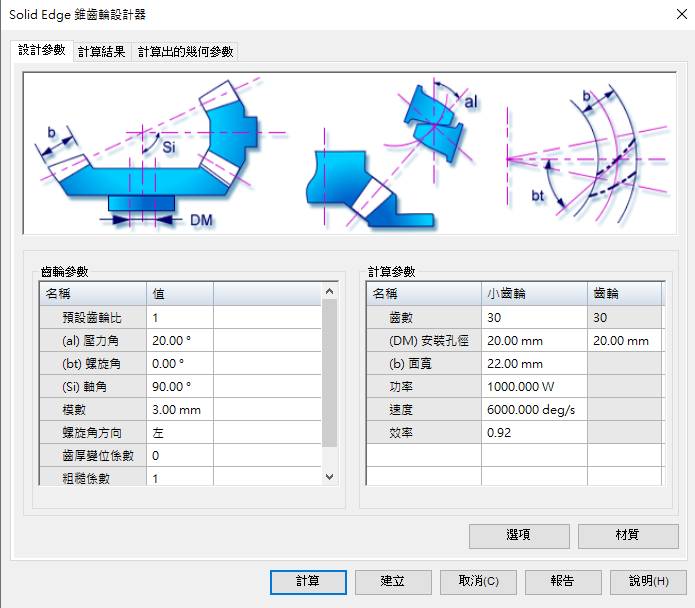
\includegraphics[width=12cm]{錐齒輪1}
		\caption{\Large 錐齒輪設計器}\label{2.25}
		\end{center}
		\end{figure}
		\\
		選項(圖.\ref{2.26}) \\
		\qquad 能調整要計算的分析選項及結果\\
		\begin{figure}[hbt!]
		\begin{center}
		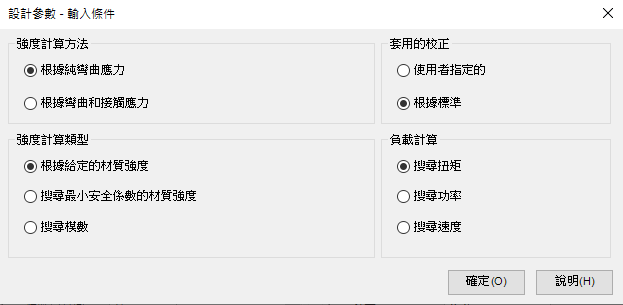
\includegraphics[width=10cm]{錐齒輪2}
		\caption{\Large 設計參數選項}\label{2.26}
		\end{center}
		\end{figure}
		\\
		材質(圖.\ref{2.27}) \\
		材質的設定\\
		\begin{figure}[hbt!]
		\begin{center}
		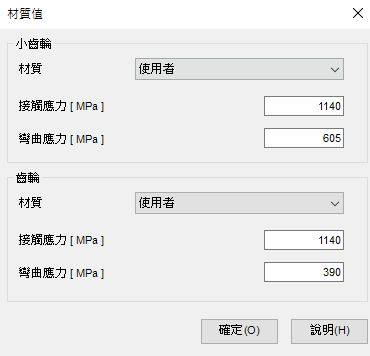
\includegraphics[width=8cm]{錐齒輪3}
		\caption{\Large 錐齒輪材質}\label{2.27}
		\end{center}
		\end{figure}
		\\
		計算結果(圖.\ref{2.28}) \\
		\qquad 設計計算後的分析結果\\
		\begin{figure}[hbt!]
		\begin{center}
		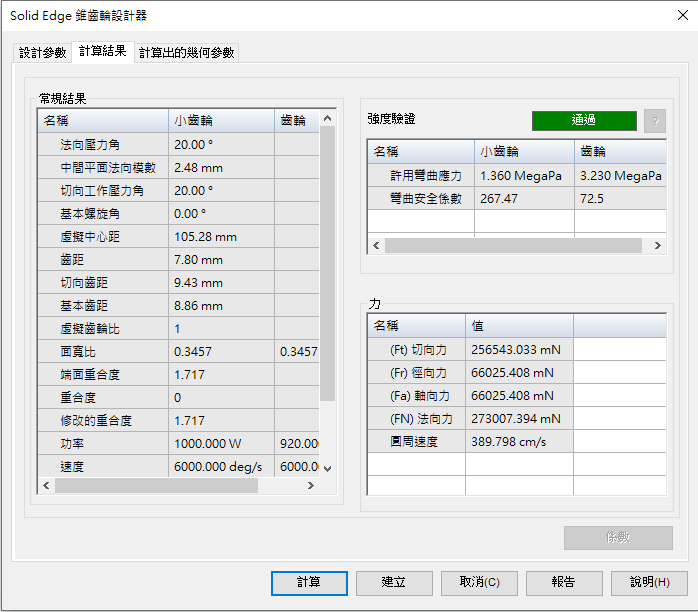
\includegraphics[width=12cm]{錐齒輪4}
		\caption{\Large 錐齒輪計算結果}\label{2.28}
		\end{center}
		\end{figure}
		\\
		計算出的幾何參數(圖.\ref{2.29}) \\
		\qquad 根據設計參數所生成之錐齒輪的各細項尺寸\\
		\begin{figure}[hbt!]
		\begin{center}
		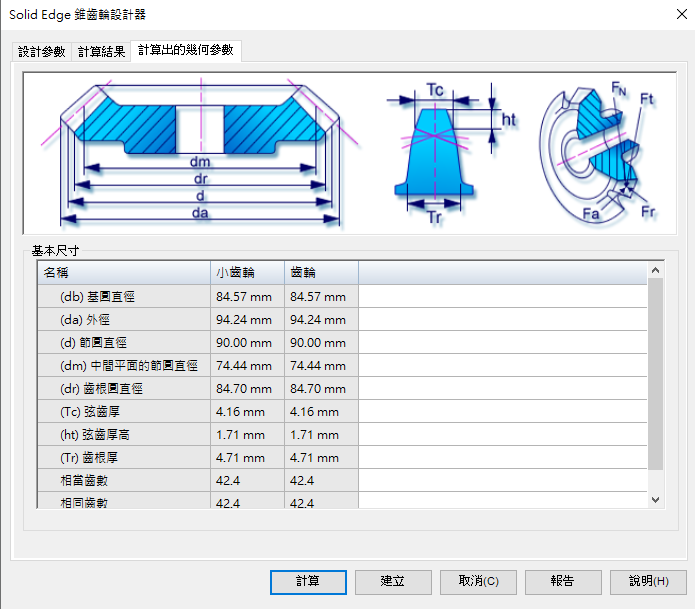
\includegraphics[width=12cm]{錐齒輪5}
		\caption{\Large 錐齒輪幾何參數}\label{2.29}
		\end{center}
		\end{figure}
		\\
		建立模型(圖.\ref{2.228}) \\
		\begin{figure}[hbt!]
		\begin{center}
		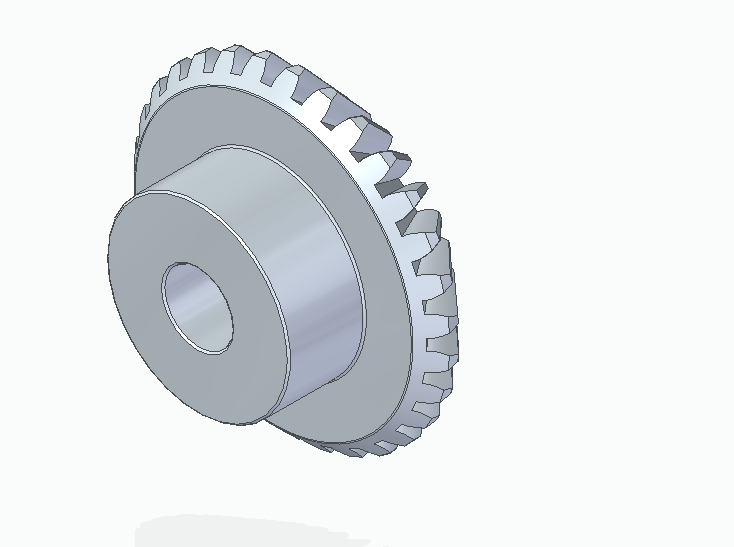
\includegraphics[width=10cm]{錐齒輪模型}
		\caption{\Large 錐齒輪模型}\label{2.228}
		\end{center}
		\end{figure}
		\\
	
\newpage	
	
	\item 渦輪設計器(圖.\ref{2.30}) :\\
		\qquad 有預設的組立件尺寸供使用者直接選擇\\
		\begin{figure}[hbt!]
		\begin{center}
		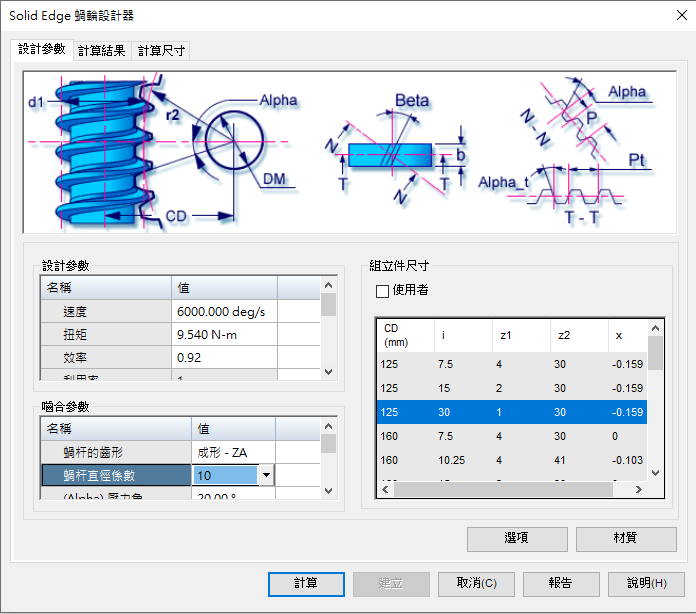
\includegraphics[width=12cm]{渦輪1}
		\caption{\Large 渦輪設計器}\label{2.30}
		\end{center}
		\end{figure}
		\\
		選項(圖.\ref{2.31}) \\
		\qquad 更細部的各項設定\\
		\begin{figure}[hbt!]
		\begin{center}
		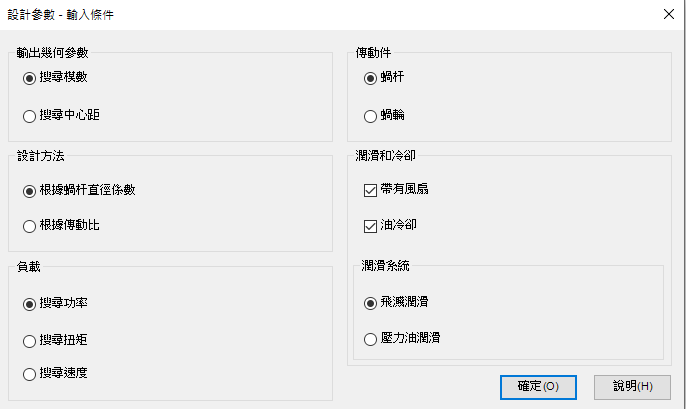
\includegraphics[width=10cm]{渦輪2}
		\caption{\Large 渦桿渦輪細部選項}\label{2.31}
		\end{center}
		\end{figure}
		\\
		材質(圖.\ref{2.32}) \\
		\qquad 渦桿與渦輪的材質設定\\
		\begin{figure}[hbt!]
		\begin{center}
		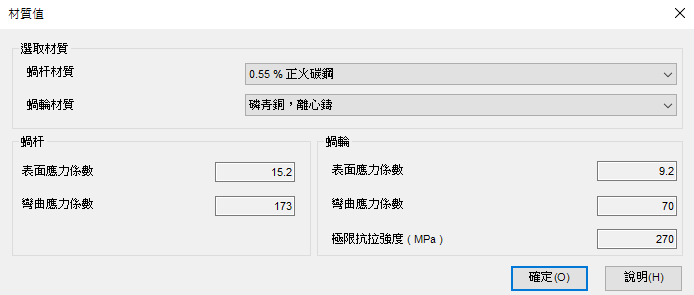
\includegraphics[width=10cm]{渦輪3}
		\caption{\Large 渦桿渦輪材質}\label{2.32}
		\end{center}
		\end{figure}
		\\
		計算結果(圖.\ref{2.33}) \\
		\qquad 設計計算後的分析結果\\
		\begin{figure}[hbt!]
		\begin{center}
		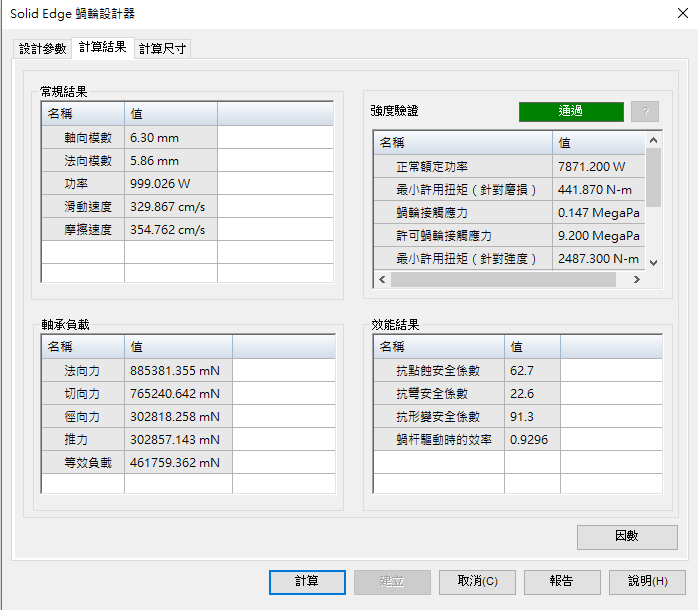
\includegraphics[width=12cm]{渦輪4}
		\caption{\Large 渦桿渦輪計算結果}\label{2.33}
		\end{center}
		\end{figure}
		\\
		係數(圖.\ref{2.34}) \\
		\qquad 計算後結果的各項係數\\
		\begin{figure}[hbt!]
		\begin{center}
		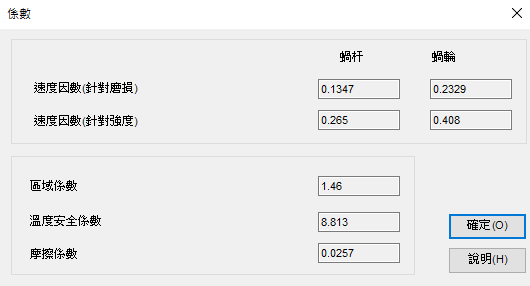
\includegraphics[width=10cm]{渦輪5}
		\caption{\Large 計算結果係數}\label{2.34}
		\end{center}
		\end{figure}
		\\
		計算尺寸(圖.\ref{2.35}) \\
		\qquad 根據設計參數所生成之渦輪的各細項尺寸\\
		\begin{figure}[hbt!]
		\begin{center}
		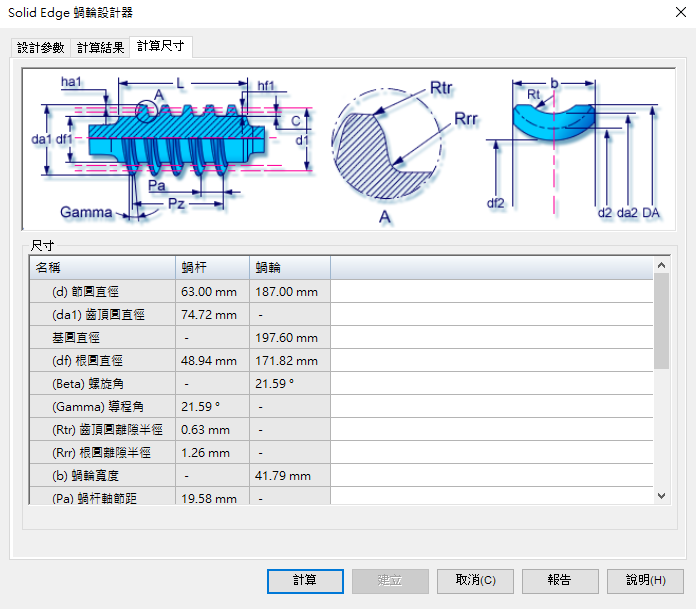
\includegraphics[width=12cm]{渦輪6}
		\caption{\Large 計算結果尺寸}\label{2.35}
		\end{center}
		\end{figure}
		\\
		建立模型(圖.\ref{2.36}、圖.\ref{2.37}) \\
		\begin{figure}[hbt!]
		\begin{center}
		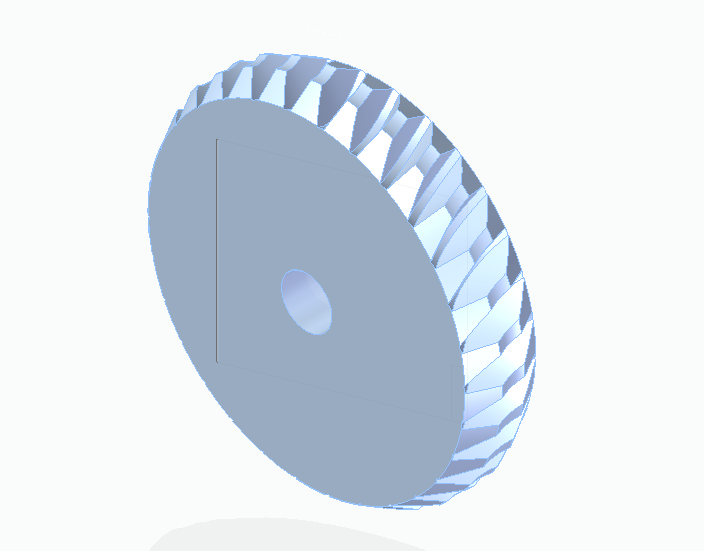
\includegraphics[width=10cm]{渦輪模型}
		\caption{\Large 渦輪模型}\label{2.36}
		\end{center}
		\end{figure}
		\\
		\begin{figure}[hbt!]
		\begin{center}
		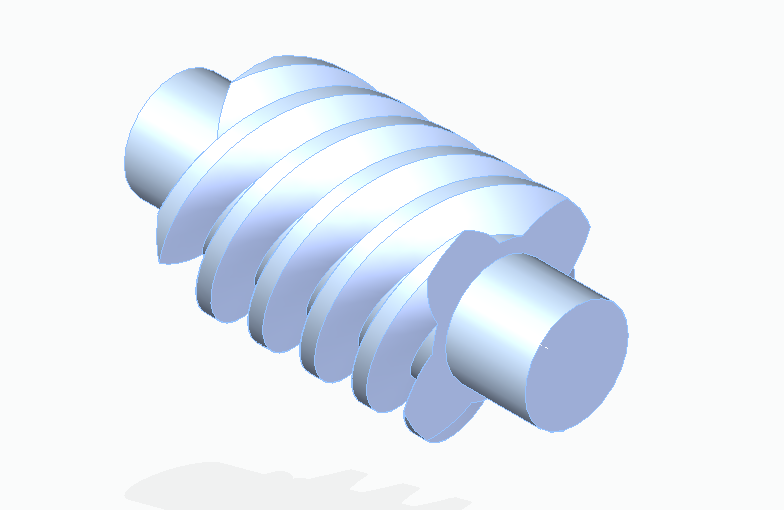
\includegraphics[width=10cm]{渦桿模型}
		\caption{\Large 渦桿模型}\label{2.37}
		\end{center}
		\end{figure}
		\\
\newpage
	\item 齒輪齒條傳動裝置設計器(圖.\ref{2.38}) \\
		\qquad 齒輪與齒條的代號介紹及尺寸設定\\
		\begin{figure}[hbt!]
		\begin{center}
		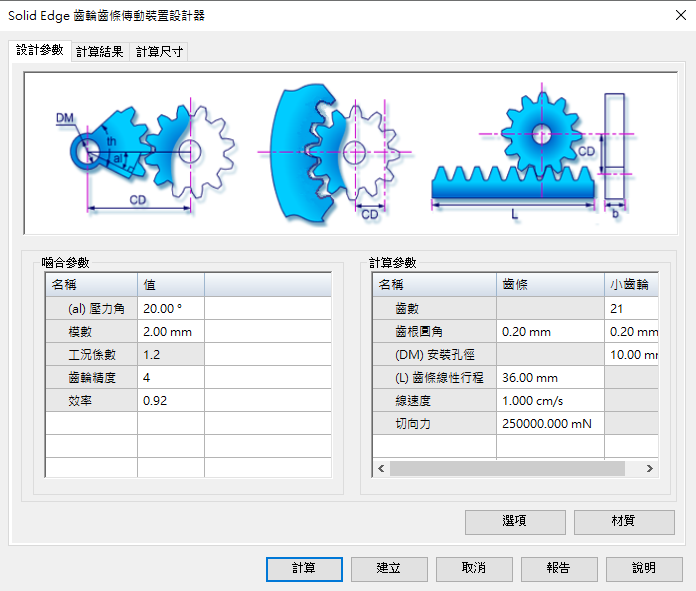
\includegraphics[width=12cm]{齒輪齒條1}
		\caption{\Large 齒輪齒條傳動裝置設計器}\label{2.38}
		\end{center}
		\end{figure}
		\\
		選項(圖.\ref{2.39}) \\
		\qquad 設定尺條類型及計算條件\\
		\begin{figure}[hbt!]
		\begin{center}
		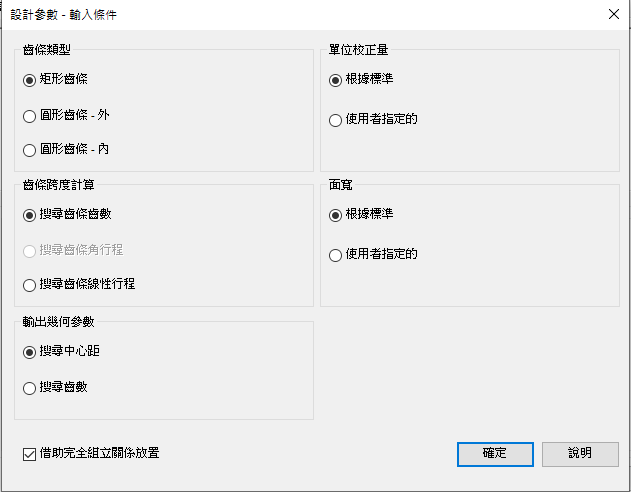
\includegraphics[width=8cm]{齒輪齒條2}
		\caption{\Large 齒輪齒條材質}\label{2.39}
		\end{center}
		\end{figure}
		\\
		材質(圖.\ref{2.40}) \\
		\qquad 齒輪齒條的材質設定\\
		\begin{figure}[hbt!]
		\begin{center}
		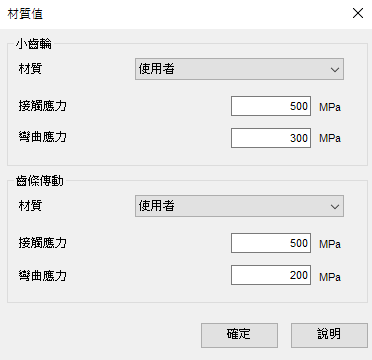
\includegraphics[width=8cm]{齒輪齒條3}
		\caption{\Large 齒輪齒條材質}\label{2.40}
		\end{center}
		\end{figure}
		\\
		計算結果(圖.\ref{2.41}) \\
		\qquad 依照參數設定計算出的結果\\
		\begin{figure}[hbt!]
		\begin{center}
		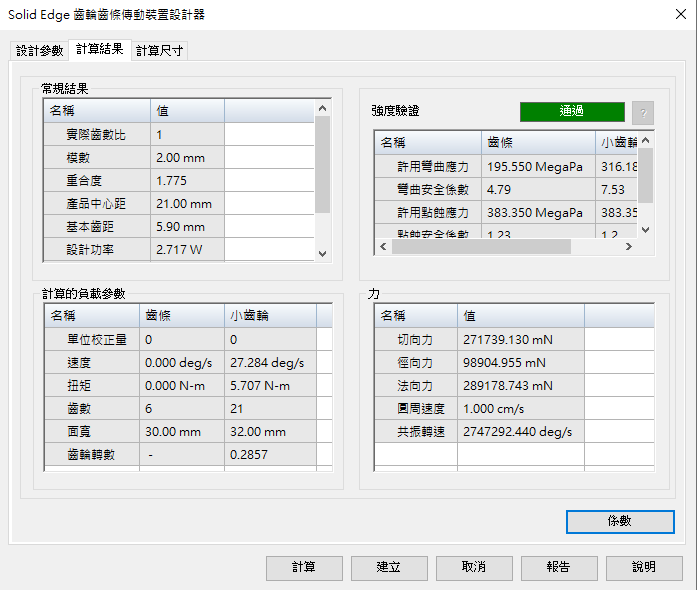
\includegraphics[width=12cm]{齒輪齒條4}
		\caption{\Large 齒輪齒條計算結果}\label{2.41}
		\end{center}
		\end{figure}
		\\
		係數(圖.\ref{2.42}) \\
		\qquad 計算結果的各項係數\\
		\begin{figure}[hbt!]
		\begin{center}
		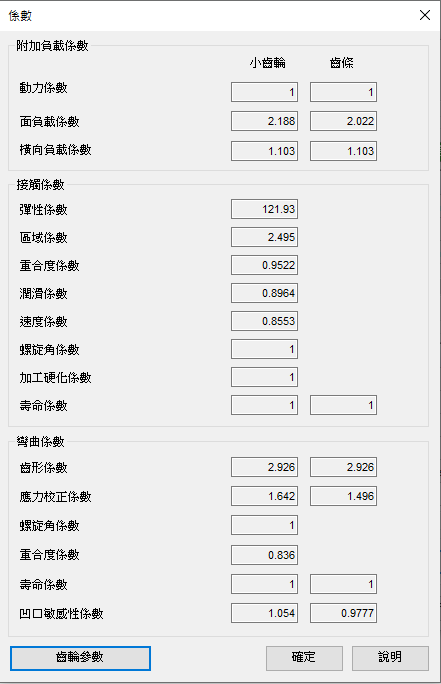
\includegraphics[width=8cm]{齒輪齒條5}
		\caption{\Large 計算結果係數}\label{2.42}
		\end{center}
		\end{figure}
		\\
		齒輪參數(圖.\ref{2.43}) \\
		\qquad 根據設計參數所生成之齒輪與齒條的各細項尺寸\\
		\begin{figure}[hbt!]
		\begin{center}
		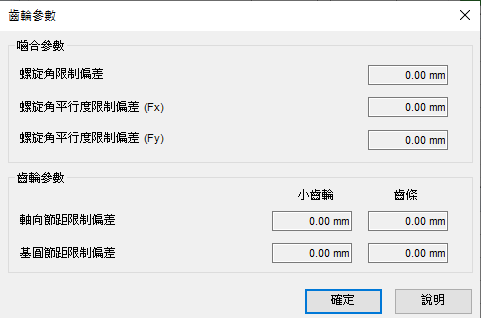
\includegraphics[width=10cm]{齒輪齒條6}
		\caption{\Large 齒輪齒條材質}\label{2.43}
		\end{center}
		\end{figure}
		\\
		計算尺寸(圖.\ref{2.431}) \\
		\qquad 根據設計參數所生成之齒輪與齒條的各細項尺寸\\
		\begin{figure}[hbt!]
		\begin{center}
		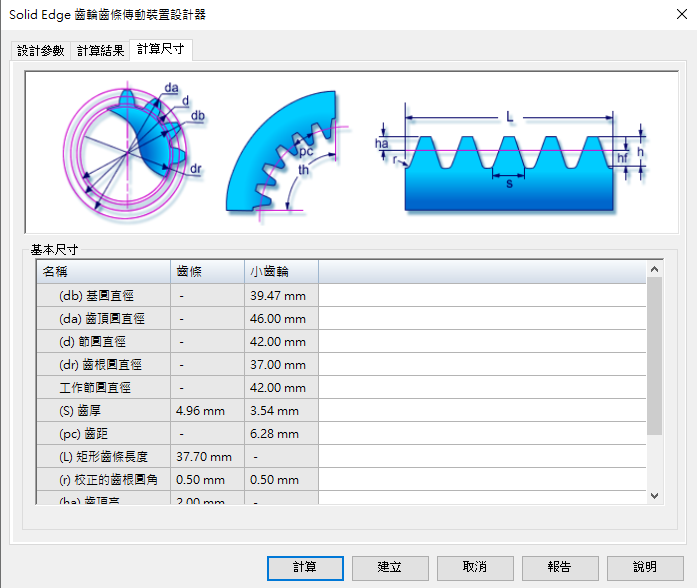
\includegraphics[width=12cm]{齒輪齒條7}
		\caption{\Large 齒輪齒條材質}\label{2.431}
		\end{center}
		\end{figure}
		\\
		模型建立(圖.\ref{2.44}、圖.\ref{2.45}) \\
		\begin{figure}[hbt!]
		\begin{center}
		\includegraphics[width=10cm]{齒輪齒條1模型}
		\caption{\Large 齒輪模型}\label{2.44}
		\end{center}
		\end{figure}
		\\
		\begin{figure}[hbt!]
		\begin{center}
		\includegraphics[width=10cm]{齒輪齒條2模型}
		\caption{\Large 齒條模型}\label{2.45}
		\end{center}
		\end{figure}
		\\
		
	\item 鍊輪設計器(圖.\ref{2.46}) : \\
		\qquad 鍊條與鍊輪的參數設定\\
		\begin{figure}[hbt!]
		\begin{center}
		\includegraphics[width=12cm]{鍊輪1}
		\caption{\Large 鍊輪設計器}\label{2.46}
		\end{center}
		\end{figure}
		\\
		選項(圖.\ref{2.47})\\
		\qquad 設計參數的輸入條件\\
		\begin{figure}[hbt!]
		\begin{center}
		\includegraphics[width=8cm]{鍊輪2}
		\caption{\Large 鍊輪細部選項}\label{2.47}
		\end{center}
		\end{figure}
		\\
		計算結果(圖.\ref{2.48})\\
		\qquad 參數設計的計算分析結果\\
		\begin{figure}[hbt!]
		\begin{center}
		\includegraphics[width=12cm]{鍊輪3}
		\caption{\Large 鍊輪計算結果}\label{2.48}
		\end{center}
		\end{figure}
		\\
		計算尺寸(圖.\ref{2.49})\\
		\qquad 根據設計參數所生成之鍊輪的各細項尺寸,齒輪尺寸有最大與最小值之分\\
		\begin{figure}[hbt!]
		\begin{center}
		\includegraphics[width=12cm]{鍊輪4}
		\caption{\Large 鍊輪計算結果}\label{2.49}
		\end{center}
		\end{figure}
		\\
		模型建立(圖.\ref{2.50})\\
		\begin{figure}[hbt!]
		\begin{center}
		\includegraphics[width=10cm]{鏈輪模型}
		\caption{\Large 鍊輪模型}\label{2.50}
		\end{center}
		\end{figure}
		\\
		
		
	\item 壓縮彈簧設計器(圖.\ref{2.51}) :\\
		\qquad 壓縮彈簧的尺寸設定\\
		\begin{figure}[hbt!]
		\begin{center}
		\includegraphics[width=12cm]{壓縮彈簧1}
		\caption{\Large 壓縮彈簧設計器}\label{2.51}
		\end{center}
		\end{figure}
		\\
		選項(圖.\ref{2.52})\\
		\qquad 參數輸入條件\\
		\begin{figure}[hbt!]
		\begin{center}
		\includegraphics[width=10cm]{壓縮彈簧2}
		\caption{\Large 壓縮彈簧細部選項}\label{2.52}
		\end{center}
		\end{figure}
		\\
		材質(圖.\ref{2.53})\\
		\qquad 壓縮彈簧材質設定\\
		\begin{figure}[hbt!]
		\begin{center}
		\includegraphics[width=10cm]{壓縮彈簧3}
		\caption{\Large 壓縮彈簧材質}\label{2.53}
		\end{center}
		\end{figure}
		\\
		計算結果(圖.\ref{2.54})\\
		\qquad 根據設計參數所生成之拉伸彈簧的各細項尺寸\\
		\begin{figure}[hbt!]
		\begin{center}
		\includegraphics[width=12cm]{壓縮彈簧4}
		\caption{\Large 壓縮彈簧計算結果}\label{2.54}
		\end{center}
		\end{figure}
		\\
		模型建立(圖.\ref{2.55})\\
		\begin{figure}[hbt!]
		\begin{center}
		\includegraphics[width=10cm]{壓縮彈簧模型}
		\caption{\Large 壓縮彈簧模型}\label{2.55}
		\end{center}
		\end{figure}
		\\
		
\newpage
		
	\item 拉伸彈簧設計器(圖.\ref{2.56}) :\\
		\qquad 拉伸彈簧尺寸輸入\\
		\begin{figure}[hbt!]
		\begin{center}
		\includegraphics[width=12cm]{拉伸彈簧1}
		\caption{\Large 拉伸彈簧設計器}\label{2.56}
		\end{center}
		\end{figure}
		\\
		選項(圖.\ref{2.57})\\
		\qquad 參數輸入條件\\
		\begin{figure}[hbt!]
		\begin{center}
		\includegraphics[width=10cm]{拉伸彈簧2}
		\caption{\Large 拉伸彈簧細部選項}\label{2.57}
		\end{center}
		\end{figure}
		\\
		材質(圖.\ref{2.58})\\
		\qquad 拉伸彈簧材料設定\\
		\begin{figure}[hbt!]
		\begin{center}
		\includegraphics[width=8cm]{拉伸彈簧3}
		\caption{\Large 拉伸彈簧材質}\label{2.58}
		\end{center}
		\end{figure}
		\\
		計算結果(圖.\ref{2.59})\\
		\qquad 根據設計參數所生成之拉伸彈簧的各細項尺寸\\
		\begin{figure}[hbt!]
		\begin{center}
		\includegraphics[width=12cm]{拉伸彈簧4}
		\caption{\Large 拉伸彈簧計算結果}\label{2.59}
		\end{center}
		\end{figure}
		\\
		模型建立(圖.\ref{2.60})\\
		\begin{figure}[hbt!]
		\begin{center}
		\includegraphics[width=10cm]{拉伸彈簧模型}
		\caption{\Large 拉伸彈簧模型}\label{2.60}
		\end{center}
		\end{figure}
		\\
		
\newpage
		
	\item 同步帶輪設計器(圖.\ref{2.61}) :\\
		\qquad 同步帶輪尺寸輸入\\
		\begin{figure}[hbt!]
		\begin{center}
		\includegraphics[width=12cm]{同步帶輪1}
		\caption{\Large 同步帶輪設計器}\label{2.61}
		\end{center}
		\end{figure}
		\\
		選項(圖.\ref{2.62}) :\\
		\qquad 參數輸入條件\\
		\begin{figure}[hbt!]
		\begin{center}
		\includegraphics[width=10cm]{同步帶輪2}
		\caption{\Large 同步帶輪細部選項}\label{2.62}
		\end{center}
		\end{figure}
		\\
		計算結果(圖.\ref{2.63}) :\\
		\qquad 計算後結果的各項係數\\
		\begin{figure}[hbt!]
		\begin{center}
		\includegraphics[width=12cm]{同步帶輪3}
		\caption{\Large 同步帶輪計算結果}\label{2.63}
		\end{center}
		\end{figure}
		\\
		計算尺寸(圖.\ref{2.64}) :\\
		\qquad 根據設計參數所生成之同步帶輪的各細項尺寸\\
		\begin{figure}[hbt!]
		\begin{center}
		\includegraphics[width=12cm]{同步帶輪4}
		\caption{\Large 計算結果尺寸}\label{2.64}
		\end{center}
		\end{figure}
		\\
		模型建立(圖.\ref{2.65}) :\\
		\begin{figure}[hbt!]
		\begin{center}
		\includegraphics[width=10cm]{同步帶輪模型}
		\caption{\Large 同步帶輪模型}\label{2.65}
		\end{center}
		\end{figure}
		\\
		
\newpage
		
	\item 帶輪設計器(圖.\ref{2.66}) :\\
		\qquad 帶輪的尺寸輸入\\
		\begin{figure}[hbt!]
		\begin{center}
		\includegraphics[width=10cm]{帶輪1}
		\caption{\Large 同步帶輪模型}\label{2.66}
		\end{center}
		\end{figure}
		\\
		選項(圖.\ref{2.67}) :\\
		\qquad 參數輸入條件\\
		\begin{figure}[hbt!]
		\begin{center}
		\includegraphics[width=10cm]{帶輪2}
		\caption{\Large 帶輪細部選項}\label{2.67}
		\end{center}
		\end{figure}
		\\
		計算結果(圖.\ref{2.68}) :\\
		\qquad 設計計算後的分析結果\\
		\begin{figure}[hbt!]
		\begin{center}
		\includegraphics[width=10cm]{帶輪3}
		\caption{\Large 帶輪計算結果}\label{2.68}
		\end{center}
		\end{figure}
		\\
		計算尺寸(圖.\ref{2.69}) :\\
		\qquad 根據設計參數所生成之帶輪的各細項尺寸\\
		\begin{figure}[hbt!]
		\begin{center}
		\includegraphics[width=10cm]{帶輪4}
		\caption{\Large 計算結果尺寸}\label{2.69}
		\end{center}
		\end{figure}
		\\
		模型建立(圖.\ref{2.70}) :\\
		\begin{figure}[hbt!]
		\begin{center}
		\includegraphics[width=10cm]{帶輪模型}
		\caption{\Large 計算結果尺寸}\label{2.70}
		\end{center}
		\end{figure}
		\\
		
	\item 樑設計器(圖.\ref{2.71}) :\\
		\qquad 樑的尺寸輸入,與軸設計器相同有設計的預覽畫面\\
		\begin{figure}[hbt!]
		\begin{center}
		\includegraphics[width=12cm]{樑1}
		\caption{\Large 樑設計器}\label{2.71}
		\end{center}
		\end{figure}
		\\
		材質(圖.\ref{2.72}) :\\
		\qquad 樑的材料設定\\
		\begin{figure}[hbt!]
		\begin{center}
		\includegraphics[width=10cm]{樑2}
		\caption{\Large 樑材質}\label{2.72}
		\end{center}
		\end{figure}
		\\
		計算結果(圖.\ref{2.73}) :\\
		\qquad 設計計算後的分析結果,根據圖形選項得到不同的作用力\\
		\begin{figure}[hbt!]
		\begin{center}
		\includegraphics[width=12cm]{樑3}
		\caption{\Large 樑計算結果}\label{2.72}
		\end{center}
		\end{figure}
		\\
		模型建立(圖.\ref{2.73}) :\\
		\begin{figure}[hbt!]
		\begin{center}
		\includegraphics[width=10cm]{樑模型}
		\caption{\Large 樑模型}\label{2.73}
		\end{center}
		\end{figure}
		\\
		
	\item 柱設計器(圖.\ref{2.74}) :\\
		\qquad 柱的尺寸輸入\\
		\begin{figure}[hbt!]
		\begin{center}
		\includegraphics[width=12cm]{柱1}
		\caption{\Large 桿設計器}\label{2.74}
		\end{center}
		\end{figure}
		\\
		選項(圖.\ref{2.75}) :\\
		\qquad 樑的設計準則\\
		\begin{figure}[hbt!]
		\begin{center}
		\includegraphics[width=10cm]{柱2}
		\caption{\Large 桿設計準則}\label{2.75}
		\end{center}
		\end{figure}
		\\
		材質(圖.\ref{2.76}) :\\
		\qquad 樑的材質設定\\
		\begin{figure}[hbt!]
		\begin{center}
		\includegraphics[width=10cm]{柱3}
		\caption{\Large 桿材質}\label{2.76}
		\end{center}
		\end{figure}
		\\
		計算結果(圖.\ref{2.77}) :\\
		\qquad 設計計算後的分析結果\\
		\begin{figure}[hbt!]
		\begin{center}
		\includegraphics[width=12cm]{柱4}
		\caption{\Large 桿計算結果}\label{2.77}
		\end{center}
		\end{figure}
		\\
		模型建立(圖.\ref{2.78}) :\\
		\begin{figure}[hbt!]
		\begin{center}
		\includegraphics[width=12cm]{柱模型}
		\caption{\Large 桿模型}\label{2.78}
		\end{center}
		\end{figure}
		\\
\end{itemize}

\newpage

\section{有限元素分析}

\subsection{有限元素法}

有限元素法(Finite element method),簡單來說就是使用有限元素分析物理現象,是一種用於求解微分方程組或積分方程組數值解的數值方法。\\

在解偏微分方程的過程中,主要難點是如何構造一個方程來逼近原本研究的方程,並且該過程還需要保持數值穩定性。目前有許多處理的方法,他們各有利弊。當區域改變時(就像一個邊界可變的固體),當需要的精確度在整個區域上變化,或者當解缺少光滑性時,有限元方法是在複雜區域(像汽車、船體結構、輸油管道)上解偏微分方程的一個很好的選擇。\\

為了解決問題,有限元素法將大型物理系統細分為更小、更簡單的部分,稱為有限元(finite element)。\\

這是通過在空間維度上進行特定的空間離散化來實現的,該離散化是通過構建對象的網格實現的:解決方案的數值域具有有限數量的點。邊值問題的有限元素法公式化最終形成了一個代數方程組。該方法在域上近似未知函數。然後將對這些有限元建模的簡單方程式組合成一個對整個問題進行建模的較大方程式系統。有限元素法通過最小化關聯的誤差函數,使用來自變異演算的變異方法來近似求解。\\

將整個物理系統細分為更簡單的部分具有以下優點:\\
\begin{itemize}
\item 精確表示複雜的幾何形狀。\\
\item 可以描述多樣的材料特性。\\
\item 輕鬆表示整體解決方案。\\
\item 精確描述局部現象。\\

該方法的工作流程包括:\\

1.將問題的域劃分為子域的集合,每個子域由一組元素方程表示為原始問題\\

2.系統地將所有元素方程組重組為用於最終計算的全域方程組。\\

\qquad 在上面的第一步中,元素方程是簡化過的方程,可以局部地近似要研究的原始復雜方程組,其中原始方程通常是偏微分方程。為了求此方程式的近似解,通常將有限元素法作為伽遼金法的特例來處理。\\

\qquad 用數學語言來說,該過程是將殘差和加權函數取內積,並將該積分設為零。簡而言之,它是通過將試驗函數擬合到偏微分方程中來最小化近似誤差的過程。殘差是由試驗函數引起的誤差,權重函數是投影殘差的多項式逼近函數。該過程消除了偏微分方程中的所有空間導數,從而使偏微分方程局部近似為一組穩態問題的代數方程,或是一組用於瞬態問題的常微分方程。如果基礎偏微分方程是線性的,則元素方程也是線性的,反之亦然。\\

\qquad 穩態問題中出現的代數方程組,便利用數值線性代數方法求解,而瞬態問題中出現的常微分方程組則使用其他數值方法(例如歐拉方法或Runge-Kutta法)通過數值積分來求解。\\

\qquad 由研究人員建立的有限元素網格,然後使用套裝軟體找到解決磁性問題的方法。 顏色表示分析人員已為每個區域設置了材料屬性,在圖\ref{2.84}中,淺藍色的鐵磁成分,淺紫色的是空氣。\\
\begin{figure}[hbt!]
\begin{center}
\includegraphics[width=8cm]{有限元素mash1}
\caption{\Large 有限元素網格1}\label{2.84}
\end{center}
\end{figure}
\\
\qquad 有限元素法解決左側問題的方法,涉及電磁屏蔽。 磁性圓筒形遮蔽罩保護內部區域不受外部磁場影響。 如圖\ref{2.85}所示,顏色表示磁場的強度,紅色為高強度磁場。 圓柱體內部的區域是低強度的(深藍色,具有寬間隔的磁通量線),這表明遮蔽罩的性能達到了設計目標。\\
\begin{figure}[hbt!]
\begin{center}
\includegraphics[width=8cm]{有限元素mash2}
\caption{\Large 有限元素網格2}\label{2.85}
\end{center}
\end{figure}
\\
\subsection{有限元概念}

\item 元素\

\qquad 元素(Element)是由節點組成的幾何體,如三角形元素,四面體元素等。 \\
\item 節點\\

\qquad 節點(Node)是元素幾何體的端點、頂點或特定點,元素的各物理量變化均體現在節點上,例如在彈性力學問題中,一個有兩個節點的線元素的質量集中在兩個節點上,受力也只能作用在節點上,變形也用節點的位移表示。 \\
\item 自由度\\

\qquad 節點自由度(Degree of Freedom,簡寫 DoF),是節點上變量的個數,例如用位移法解結構問題時節點自由度為3,表示單個節點上三個坐標方向上的位移,又例如熱分析時節點自由度為1,表示某個節點處的溫度值。 \\
\item 網格\\

\qquad 網格(Mesh)是由多個元素通過共用節點組成的元素網絡,用以表示待解問題域。 \\

\subsection{分析方法}

\qquad 以下用有限元分析解決兩個簡單問題,更一般的問題可以類似的推導出來。\\
\qquad P1是一個較簡單的一維問題 \\
\begin{figure}[hbt!]
\begin{center}
\includegraphics[width=6cm]{有限元素函數P1}
\end{center}
\end{figure}
\\

\qquad 其中$ f$是已知函數,$ u$是關於$ x$的未知函數,$ u ″$是$ u$對$ x$的二階導數。\\
二維比較簡單的問題是狄利克雷問題 \\
\begin{figure}[hbt!]
\begin{center}
\includegraphics[width=9cm]{有限元素函數P2}
\end{center}
\end{figure}
\\

\qquad 其中$\Omega$ 是$ (x,y)$平面上的連通開區域,它的邊界$ \partial $ $\Omega$ 是良好的(例如,光滑流形或多邊形),$ u_{{xx}}$和$ u_{{yy}}$分別表示 $ x$和$ y$的二階導數。問題P1能夠通過計算不定積分而直接解決。然而,解決邊值問題的這一方法只有在空間維數為1時才可用,並且不能推廣到高維問題以及形如 $u+u''=f$的問題。出於這種考慮,我們將用有限元方法解決P1並將其推廣至問題P2。\\ 
\qquad 我們的描述分為兩步,每步都反映了用有限元解決邊值問題的本質。 \\
\item 將原問題描述為它的弱形式,或變分形式。這一步很少或不需要計算。\\
\item 離散化,將弱形式在有限維空間離散化。\\

\qquad 這兩步之後,我們可以構造一個大型有限維線性方程,線性方程的解就是原邊值問題的逼近解。然後,這一有限維問題由計算機求解。 \\

\subsection{弱解形式}
\item P1的弱解形式\\

\qquad 第一步是將問題P1和P2轉化為他的等價變分形式,或弱解形式。如果 u是問題P1的解,那麼對任何滿足邊界條件的光滑函數 v ,有 \\
\begin{figure}[hbt!]
\begin{center}
\includegraphics[width=10cm]{有限元素函數3}
\end{center}
\end{figure}
\\

\qquad 相反如果$ u$對任何光滑函數$ v(x)$滿足$ u(0)=u(1)=0$和(1),\\

\qquad 那麼 u u是P1的解。對於二次可導函數 u u證明這一點是非常容易的(利用中值定理)。\\

\qquad 通過對(1)的右側使用分部積分,可以得到 \\
\begin{figure}[hbt!]
\begin{center}
\includegraphics[width=9cm]{有限元素函數4}
\end{center}
\end{figure}
\\
其中假設$ v(0)=v(1)=0$。\\

\item P2的弱解形式\\

\qquad $ f$當我們使用格林恆等式來表示式(2), P2可以$ u$的積分型式表示,在此定義$ {\displaystyle \phi (u,v)} $\\
\begin{figure}[hbt!]
\begin{center}
\includegraphics[width=9cm]{有限元素函數5}
\end{center}
\end{figure}
\\

\qquad 此處 $ \nabla$ 代表梯度,即為二維平面上的內積 。另外$ {\displaystyle \,\!\phi }$可以轉為內積空間$ {\displaystyle H_{0}^{1}(\Omega )}$ ,且$ \Omega$ 的一次微分函數$ \partial \Omega$ 為零。我們也可以假設$ {\displaystyle v\in H_{0}^{1}(\Omega )}$(詳見索伯列夫空間)也可以顯示解的存在性和唯一性。\\ 

\subsection{離散化}

\qquad P1 和 P2 通過上述過程被離散化,並簡化為子問題。 基本思路是將無限維線性問題替換掉:\\

    找到$ {\displaystyle u\in H_{0}^{1}} $使\\
	
    $ {\displaystyle \forall v\in H_{0}^{1},\;-\phi (u,v)=\int fv}$\\

表示唯有限維度的形式:\\

    子問題(3)$ {\displaystyle u\in V} $such that\\
	
    $ {\displaystyle \forall v\in V,\;-\phi (u,v)=\int fv}$\\
	
\qquad 此處$ V $是 ${\displaystyle H_{0}^{1}}$的一個有限維度線性子空間。\\

\qquad $ V$有許多可能的形式,但對於有限元素而言,在此將假定$ V$存在於分段多項式函數的空間中。 \\

對於 P1\\

\qquad 在此在區間$ (0,1)$之中選擇$ n$個$ x$的可能值$ {\displaystyle 0=x_{0}<x_{1}<\cdots <x_{n}<x_{n+1}=1}$ 接著定義$ V $為:\\

$ {\displaystyle V=\{v:[0,1]\rightarrow \mathbb {R} \;:v{\mbox{ is continuous, }}v|_{[x_{k},x_{k+1}]}{\mbox{ is linear for }}k=0,\dots ,n{\mbox{, and }}v(0)=v(1)=0\}}$\\

\qquad 令e$ x_0=0 $和$ {\displaystyle x_{n+1}=1}$。觀察到在$ V $之中的函數根據微積分的基本定義是不可微分的。 當然,當$v \in V$,則通常不定義 $ {\displaystyle x=x_{k}}$ ,${\displaystyle k=1,\ldots ,n}$的導數,但導數事實上存在於每一個$ x$的位置,並可以利用這些導數來進行部分積分運算。 \\

對於P2\\

\qquad V 是屬於$ \Omega$ 的一系列函數。 在右圖中,圖片下半部是一個15邊形的平面$ \Omega $的三角分割,以及該多邊形的分段線性函數(圖片上半部彩色部份),即 在三角分割所形成的每個三角形上呈線性; 空間$ V$則由在所在的三角分割的每個三角形上的函數線性組合而成。\\


\qquad 我們希望當下面的三角形網格變得越來越精細,離散子問題的解在某種意義上將收斂到原始邊界值問題P2的解。 為了測量此網格的細度,三角分割由一很小的實數 $ {\displaystyle h>0}$所表示。此參數將與三角分割中最大或平均三角形的大小有關。 當我們提高三角分割的精度時(分割出更多三角形),分段線性函數的空間$ V$應會隨$ h$變動。因此,在某些文獻中會以$V_{h}$來代表。 \\

\qquad 有限元素法並非全無缺點,以下圖\ref{2.90}列舉常用之三種數值方法的優劣比較,以供使用數值分析前之參考:\\
\begin{figure}[hbt!]
\begin{center}
\includegraphics[width=14cm]{數值分析}
\caption{\Large 數值分析方法之優劣比較}\label{2.90}
\end{center}
\end{figure}
\\
\end{itemize}
\newpage